%%%%%%%%%%%%%%%%%%%%%%%%%%%%%%%%%%%%%%%%%%%%%%%%%%%%%%%%%%%%%%%%%%%%%%%%%%%%%%%%%%
\begin{frame}[fragile]\frametitle{}
\begin{center}
{\Large RandomForest and Logistic Regression in credit scoring}

{\tiny (Ref: mlcourse.ai Assignment 5 – Open Machine Learning Course ) }
\end{center}

\end{frame}


%%%%%%%%%%%%%%%%%%%%%%%%%%%%%%%%%%%%%%%%%%%%%%%%%%%%%%%%%%
\begin{frame}[fragile]\frametitle{Problem Info}
Target variable: SeriousDlqin2yrs - the person had long delays in payments during 2 years; binary variable

Features:
\begin{itemize}
\item age - Age of the loan borrower 
\item NumberOfTime30-59DaysPastDueNotWorse - a delay in repaying other loans more than 30-59 days 
\item DebtRatio - monthly payments (loans, alimony, etc.) divided by aggregate monthly income, percentage
\item MonthlyIncome - monthly income in dollars
\item NumberOfTimes90DaysLate - delay in repaying other loans for more than 90 days
\item NumberOfTime60-89DaysPastDueNotWorse - a delay in repaying other loans more than 60-89 days
\item NumberOfDependents - number of people in the family
\end{itemize}
\end{frame}


%%%%%%%%%%%%%%%%%%%%%%%%%%%%%%%%%%%%%%%%%%%%%%%%%%%%%%%%%%
\begin{frame}[fragile]\frametitle{Preparation}
Import Libraries
\begin{lstlisting}
import numpy as np
import pandas as pd
import matplotlib.pyplot as plt
\end{lstlisting}
 Implement a function that will replace the NaN values by the median in each column of the table.
 \begin{lstlisting}
def impute_nan_with_median(table):
    for col in table.columns:
        table[col]= table[col].fillna(table[col].median())
    return table  
\end{lstlisting}
\end{frame}

%%%%%%%%%%%%%%%%%%%%%%%%%%%%%%%%%%%%%%%%%%%%%%%%%%%%%%%%%%
\begin{frame}[fragile]\frametitle{Read Data}
\begin{lstlisting}
data = pd.read_csv('data/credit_scoring_sample.csv', sep=",")
data.head()
\end{lstlisting}
\begin{center}
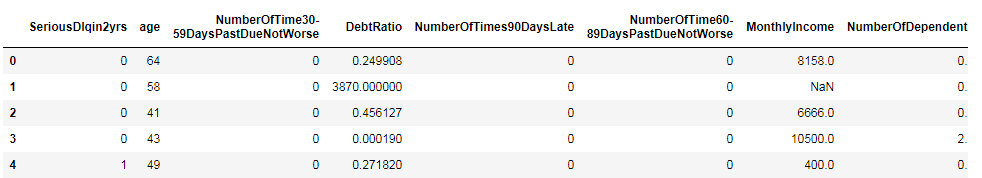
\includegraphics[width=\linewidth,keepaspectratio]{rf1}
\end{center}
\end{frame}

%%%%%%%%%%%%%%%%%%%%%%%%%%%%%%%%%%%%%%%%%%%%%%%%%%%%%%%%%%
\begin{frame}[fragile]\frametitle{Explore Data}
\begin{lstlisting}
data.dtypes

>>>
SeriousDlqin2yrs                          int64
age                                       int64
NumberOfTime30-59DaysPastDueNotWorse      int64
DebtRatio                               float64
NumberOfTimes90DaysLate                   int64
NumberOfTime60-89DaysPastDueNotWorse      int64
MonthlyIncome                           float64
NumberOfDependents                      float64
dtype: object
\end{lstlisting}
\end{frame}

%%%%%%%%%%%%%%%%%%%%%%%%%%%%%%%%%%%%%%%%%%%%%%%%%%%%%%%%%%
\begin{frame}[fragile]\frametitle{Explore Data}
Look at the distribution of classes in target:

\begin{lstlisting}
ax = data['SeriousDlqin2yrs'].hist(orientation='horizontal', color='red')
ax.set_xlabel("number_of_observations")
ax.set_ylabel("unique_value")
ax.set_title("Target distribution")

print('Distribution of target:')
data['SeriousDlqin2yrs'].value_counts() / data.shape[0]

>>>
Distribution of target:
0    0.777511
1    0.222489
Name: SeriousDlqin2yrs, dtype: float64
\end{lstlisting}
\begin{center}
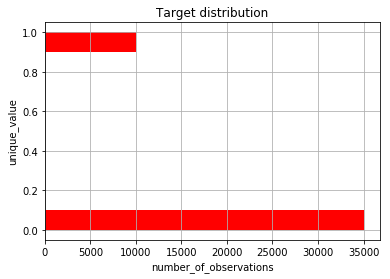
\includegraphics[width=0.3\linewidth,keepaspectratio]{rf2}
\end{center}
\end{frame}

%%%%%%%%%%%%%%%%%%%%%%%%%%%%%%%%%%%%%%%%%%%%%%%%%%%%%%%%%%
\begin{frame}[fragile]\frametitle{Prepare Data}
Select all the features and drop the target:
\begin{lstlisting}
independent_columns_names = data.columns.values
independent_columns_names = [x for x in data if x != 'SeriousDlqin2yrs']
independent_columns_names

>>>
['age',
 'NumberOfTime30-59DaysPastDueNotWorse',
 'DebtRatio',
 'NumberOfTimes90DaysLate',
 'NumberOfTime60-89DaysPastDueNotWorse',
 'MonthlyIncome',
 'NumberOfDependents']
\end{lstlisting}
\end{frame}



%%%%%%%%%%%%%%%%%%%%%%%%%%%%%%%%%%%%%%%%%%%%%%%%%%%%%%%%%%
\begin{frame}[fragile]\frametitle{Prepare Data}
We apply a function that replaces all values of NaN by the median value of the corresponding column.

\begin{lstlisting}
table = impute_nan_with_median(data)
\end{lstlisting}
Split the target and features - now we get a training sample.
\begin{lstlisting}
X = table[independent_columns_names]
y = table['SeriousDlqin2yrs']
\end{lstlisting}
\end{frame}

%%%%%%%%%%%%%%%%%%%%%%%%%%%%%%%%%%%%%%%%%%%%%%%%%%%%%%%%%%
\begin{frame}[fragile]\frametitle{Task: Bootstrap}
Make an interval estimate based on the bootstrap of the average income (MonthlyIncome) of customers who had overdue loan payments, and of those who paid in time, make 90% confidence interval. Find the difference between the lower limit of the derived interval for those who paid in time and the upper limit for those who are overdue. So, you are asked to build 90% intervals for the income of "good" customers [good_income\_lower,good\_income\_upper] and for "bad" - [bad\_income\_lower,bad\_income\_upper] and find the difference good\_income\_lower−bad\_income\_upper.

Set np.random.seed (17). Round the answer to the integer value.

\begin{itemize}
\item 344
\item 424
\item 584
\item 654
\end{itemize}

\end{frame}

%%%%%%%%%%%%%%%%%%%%%%%%%%%%%%%%%%%%%%%%%%%%%%%%%%%%%%%%%%
\begin{frame}[fragile]\frametitle{Task: Decision tree, hyperparameter tuning}
\begin{itemize}
\item One of the main performance metrics of a model is the area under the ROC curve. 
\item The ROC-AUC values lay between 0 and 1. 
\item The closer the value of ROC-AUC to 1, the better the classification is done.
\item Find the values of DecisionTreeClassifier hyperparameters using theGridSearchCV, which maximize the area under the ROC curve.
\end{itemize}


\begin{lstlisting}
from sklearn.tree import DecisionTreeClassifier
from sklearn.model_selection import GridSearchCV, StratifiedKFold
\end{lstlisting}
\end{frame}


%%%%%%%%%%%%%%%%%%%%%%%%%%%%%%%%%%%%%%%%%%%%%%%%%%%%%%%%%%
\begin{frame}[fragile]\frametitle{Hyperparameter Tuning}
\begin{itemize}
\item Use the DecisionTreeClassifier class to create a decision tree. 
\item Due to the imbalance of the classes in the target, we add the balancing parameter. 
\item We also use the parameter random\_state = 17 for the reproducibility of the results.
\end{itemize}

\begin{lstlisting}
dt = DecisionTreeClassifier(random_state=17, class_weight='balanced')
\end{lstlisting}
\end{frame}

%%%%%%%%%%%%%%%%%%%%%%%%%%%%%%%%%%%%%%%%%%%%%%%%%%%%%%%%%%
\begin{frame}[fragile]\frametitle{Task: Decision tree, hyperparameter tuning}
We will look through such values of hyperparameters:

\begin{lstlisting}
max_depth_values = [5, 6, 7, 8, 9]
max_features_values = [4, 5, 6, 7]
tree_params = {'max_depth': max_depth_values,
               'max_features': max_features_values}
\end{lstlisting}

Fix cross-validation parameters: stratified, 5 partitions with shuffle, random\_state.
\begin{lstlisting}
skf = StratifiedKFold(n_splits=5, shuffle=True, random_state=17)
\end{lstlisting}

\end{frame}

%%%%%%%%%%%%%%%%%%%%%%%%%%%%%%%%%%%%%%%%%%%%%%%%%%%%%%%%%%
\begin{frame}[fragile]\frametitle{Task: Decision tree, hyperparameter tuning}
\begin{itemize}
\item Run GridSearch with the ROC AUC metric using the hyperparameters from the tree\_params dictionary. \item What is the maximum ROC AUC value (round up to 2 decimals)? 
\item We call cross-validation stable if the standard deviation of the metric on the cross-validation is less than 1\%. 
\item Was cross-validation stable under optimal combinations of hyperparameters (i.e., providing a maximum of the mean ROC AUC value for cross-validation)?
\end{itemize}

Answer options:

\begin{itemize}
\item 0.82, no
\item 0.84, no
\item 0.82, yes
\item 0.84, yes
\end{itemize}
\end{frame}

%%%%%%%%%%%%%%%%%%%%%%%%%%%%%%%%%%%%%%%%%%%%%%%%%%%%%%%%%%
\begin{frame}[fragile]\frametitle{Task : RandomForest, hyperparameter tuning}
\begin{itemize}
\item We found the optimal hyperparameters for one tree. 
\item However it could be that these parameters are not optimal for an ensemble. Let's check this assumption with \lstinline|GridSearchCV (RandomForestClassifier (class_weight='balanced', random_state = 17) )|. 
\item Now we extend the value of max\_depth up to 15, because the trees need to be deeper in the forest (you should be aware of it from the article). 
\item What are the best values of hyperparameters now?
\end{itemize}

Answer options:

\begin{itemize}
\item max\_depth=8, max\_features=4
\item max\_depth=9, max\_features=5
\item max\_depth=10, max\_features=6
\item max\_depth=11, max\_features=7

\end{itemize}
\end{frame}

%%%%%%%%%%%%%%%%%%%%%%%%%%%%%%%%%%%%%%%%%%%%%%%%%%%%%%%%%%
\begin{frame}[fragile]\frametitle{Task : RandomForest, hyperparameter tuning}
\begin{lstlisting}
max_depth_values = range(5, 15)
max_features_values = [4, 5, 6, 7]
forest_params = {'max_depth': max_depth_values,
                'max_features': max_features_values}
\end{lstlisting}
\end{frame}

%%%%%%%%%%%%%%%%%%%%%%%%%%%%%%%%%%%%%%%%%%%%%%%%%%%%%%%%%%
\begin{frame}[fragile]\frametitle{Task : Logistic regression, hyperparameter tuning}
\begin{itemize}
\item Let's compare our results with logistic regression (we indicate class\_weight='balanced' and random\_state = 17). 
\item Do a full search by the parameter C from a wide range of values \lstinline|np.logspace(-8, 8, 17)|. 
\item Now we will build a pipeline - first apply scaling, then train the model.
\item 
Learn about the pipelines and make cross-validation. What is the best average ROC AUC? Select the closest value.
\end{itemize}

Answer options:

\begin{itemize}
\item 0.778
\item 0.788
\item 0.798
\item 0.808

\end{itemize}
\end{frame}

%%%%%%%%%%%%%%%%%%%%%%%%%%%%%%%%%%%%%%%%%%%%%%%%%%%%%%%%%%
\begin{frame}[fragile]\frametitle{Task : Logistic regression, hyperparameter tuning}
\begin{lstlisting}
from sklearn.pipeline import Pipeline
from sklearn.preprocessing import StandardScaler
from sklearn.linear_model import LogisticRegression

scaler = StandardScaler()
logit = LogisticRegression(random_state=17, class_weight='balanced')

logit_pipe = Pipeline([('scaler', scaler), ('logit', logit)])
logit_pipe_params = {'logit__C': np.logspace(-8, 8, 17)}
\end{lstlisting}
\end{frame}


%%%%%%%%%%%%%%%%%%%%%%%%%%%%%%%%%%%%%%%%%%%%%%%%%%%%%%%%%%
\begin{frame}[fragile]\frametitle{Task : Logistic regression and RandomForest on sparse features}
\begin{itemize}
\item In case of a small number of features, random forest was proved to be better than logistic regression. 
\item However, one of the main disadvantages of trees is how they work with sparse data, for example, with texts. 
\item Let's compare logistic regression and random forest in a new task. Download dataset with reviews of movies here (http://d.pr/f/W0HpZh)
\end{itemize}

\end{frame}

%%%%%%%%%%%%%%%%%%%%%%%%%%%%%%%%%%%%%%%%%%%%%%%%%%%%%%%%%%
\begin{frame}[fragile]\frametitle{Task : Logistic regression and RandomForest on sparse features}

\begin{lstlisting}
# Download data
df = pd.read_csv("data/movie_reviews_train.csv", nrows=50000)

# Split data to train and test
X_text = df["text"]
y_text = df["label"]

# Classes counts
df.label.value_counts()

>>>
1    32492
0    17508
Name: label, dtype: int64
\end{lstlisting}
\end{frame}

%%%%%%%%%%%%%%%%%%%%%%%%%%%%%%%%%%%%%%%%%%%%%%%%%%%%%%%%%%
\begin{frame}[fragile]\frametitle{Task : Logistic regression and RandomForest on sparse features}

\begin{lstlisting}
from sklearn.feature_extraction.text import CountVectorizer
from sklearn.pipeline import Pipeline

# Split on 3 folds
skf = StratifiedKFold(n_splits=3, shuffle=True, random_state=17)

# In Pipeline we will modify the text and train logistic regression
classifier = Pipeline([
    ('vectorizer', CountVectorizer(max_features=100000, ngram_range=(1, 3))),
    ('clf', LogisticRegression(random_state=17))])
\end{lstlisting}
\end{frame}

%%%%%%%%%%%%%%%%%%%%%%%%%%%%%%%%%%%%%%%%%%%%%%%%%%%%%%%%%%
\begin{frame}[fragile]\frametitle{Task : Logistic regression and RandomForest on sparse features}
For Logistic Regression: iterate parameter C with values from the list [0.1, 1, 10, 100] and find the best ROC AUC in cross-validation. Select the closest answer.

\begin{itemize}
\item 0.74
\item 0.75
\item 0.84
\item 0.85
\end{itemize}

\end{frame}

%%%%%%%%%%%%%%%%%%%%%%%%%%%%%%%%%%%%%%%%%%%%%%%%%%%%%%%%%%
\begin{frame}[fragile]\frametitle{Task : Logistic regression and RandomForest on sparse features}

\begin{lstlisting}
classifier = Pipeline([
    ('vectorizer', CountVectorizer(max_features=100000, ngram_range=(1, 3))),
    ('clf', RandomForestClassifier(random_state=17, n_jobs=-1))])

min_samples_leaf = [1, 2, 3]
max_features = [0.3, 0.5, 0.7]
max_depth = [None]
\end{lstlisting}
\end{frame}
